\subsection{Problem}
\label{subsec:problem}

Today's applications seem to be increasing in complexity over the last few years. 
Especially in the field of frontend development, the range of functions has increased \cite{kevin2018}.
The web development has transitioned from server rendered, page-reloading websites to modern, so called single page applications.

\begin{figure}[h]
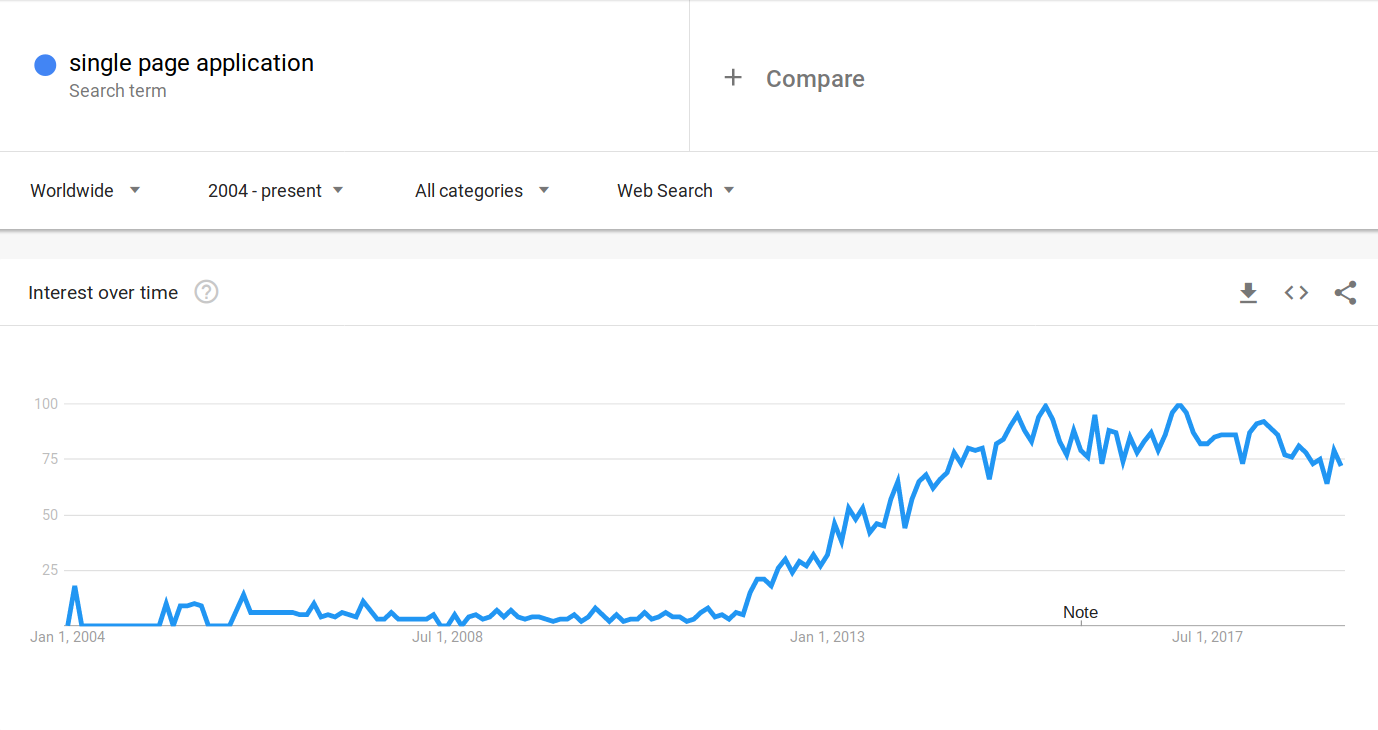
\includegraphics[width=0.97\textwidth]{google-trends-spa}
\centering
\caption{Google trends: single page application}
\label{fig:google-trends-spa}
\end{figure}

In most cases, an application communicates with other interfaces, such as a back-end or local database.
On mobile devices it's also often necessary to know the GPS status, whether mobile data is turned on off, and similar. 
A click of a user thus can cause many changes inside and outside of the application.
A developer must be aware of all the outcomes, \todo{Talk about routing/user flow/navigation} react to them and save what has happened.
He must manage the state. The problem is to find a good design pattern, which makes this task feasible.